\documentclass[11pt,a4paper]{article}  % typ papieru i rozmiar fontu
\usepackage[MeX]{polski}
\usepackage[utf8]{inputenc}
\usepackage{graphicx}
\usepackage{amsmath}
\usepackage{amssymb}
\usepackage{hyperref}
\usepackage{enumerate}

\title{na podstawie p007}
\author{Imię i nazwisko}
\date{Data ręcznie}

\begin{document}

\maketitle

\tableofcontents %spis treści

\section*{Wprowadzenie}
To jest wprowadzenie objaśniające nieco kolokwium. Zwróć uwagę, że jesteśmy w sekcji nienumerowanej. W sekcji tytułowej wpisz swoje prawdziwe
imię i nazwisko. Jako datę wpisz ręcznie datę pisania kolokwium. W tytule znajduje się specjalny symbol. Ustaw czcionkę na 11 pkt, papier jako
A4, dołącz pakiet polski. Spis treści jest na początku. Wszystkie  odsyłacze
powinny być klikalne.
\section{Sekcja 1}
Tutaj testujemy zdjęcia. Mamy parę tekstu lorem ipsum. To jest odsyłasz
do zdjęcia 1.\ref{fot:zdj}

orem ipsum dolor sit amet, consectetur adipiscing elit. Sed mattis mauris nec nisl scelerisque ultrices nec  Quisque finibus purus dui, sit amet scelerisque tellus gravida ut. Integer sit amet aliquam nunc.

 at ut nisl. Suspendisse turpis tellus, venenatis a lorem elementum, viverra iaculis lorem.

\begin{figure}[ht]
\centering
\label{fot:zdj}
        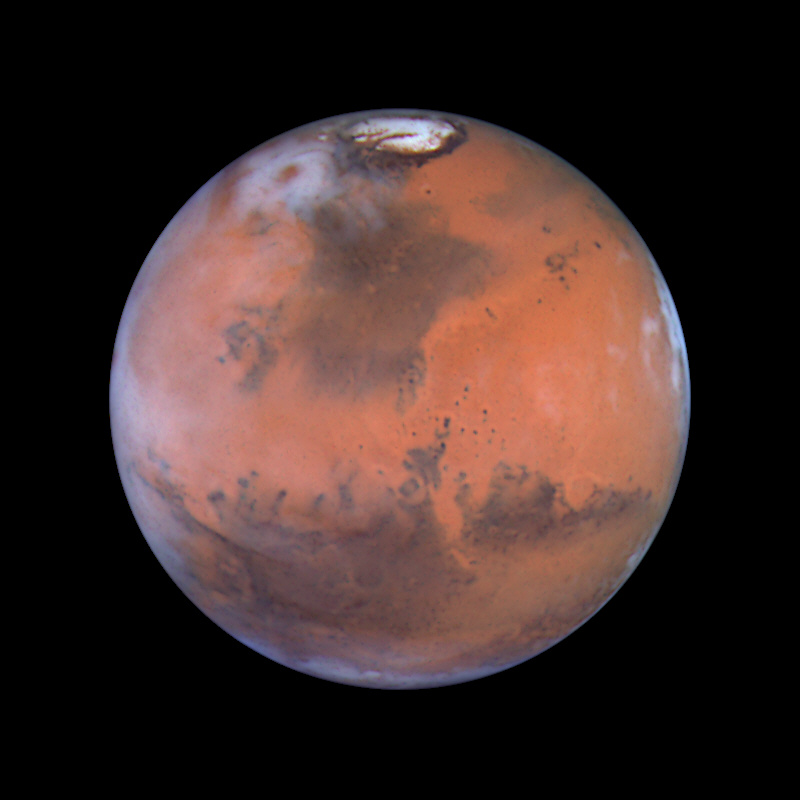
\includegraphics[width=0.3\textwidth]{mars.jpeg}
        \caption{ Ten rysunek jest w bieżącym miejscu tekstu. Szerokość to 0.3
szerokości tekstu.}
\end{figure}


Duis sapien sem, pellentesque tempor iaculis eget, gravida vel urna. Aenean varius cursus nisl, vel accumsan tellus hendrerit a. Mauris egestas turpis eu tristique varius. Phasellus condimentum commodo erat vulputate cursus. Maecenas sagittis varius tempor. Praesent rutrum, est sed imperdiet sagittis, purus justo placerat est, sit amet pulvinar nibh nulla efficitur nibh. Curabitur imperdiet hendrerit velit, ac auctor lacus congue eu. Morbi suscipit, augue nec pharetra hendrerit, nunc felis blandit nisi, a suscipit felis nulla id lectus. Integer viverra nec dolor et vulputate. Nulla at vulputate odio.


\begin{table}[]
\centering
\label{tab:tabela}

\begin{tabular}{|c|l|c|c|c|c|c|c|}
\hline
Lp. & Drużyna & M. & Pkt. & Z. & R. & P. & Bramki \\ \hline
1.  & Bruk-Bet Termalica Nieciecza        &    &      &    &    &    &        \\ \hline
2.  & Bruk-Bet Termalica Nieciecza        &    &      &    &    &    &        \\ \hline
3.  & Bruk-Bet Termalica Nieciecza       &    &      &    &    &    &        \\ \hline
4.  & Bruk-Bet Termalica Nieciecza        &    &      &    &    &    &        \\ \hline
5.  & Bruk-Bet Termalica Nieciecza        &    &      &    &    &    &        \\ \hline
6.  & Bruk-Bet Termalica Nieciecza       &    &      &    &    &    &        \\ \hline

\end{tabular}
\caption{Liga}
\end{table}

Duis varius pellentesque aliquet. Ut mattis porta odio, at fringilla dui fringilla et. Phasellus ultrices nulla dui, quis commodo odio tempus non. Curabitur aliquet laoreet dolor, porta tempor orci dignissim vitae. Pellentesque et sollicitudin augue, sed finibus metus. Praesent pretium odio nec justo volutpat, et lacinia magna eleifend. Nullam sit amet orci eu leo porttitor ultricies. Mauris lorem nulla, maximus ut nibh non, ultrices viverra enim. Praesent eget dictum nisi. Mauris rutrum, libero sed condimentum tempor, lorem augue rhoncus nibh, quis aliquet magna tortor sit amet erat. Sed id erat est. Integer pellentesque,
\begin{figure}[ht]
\centering
        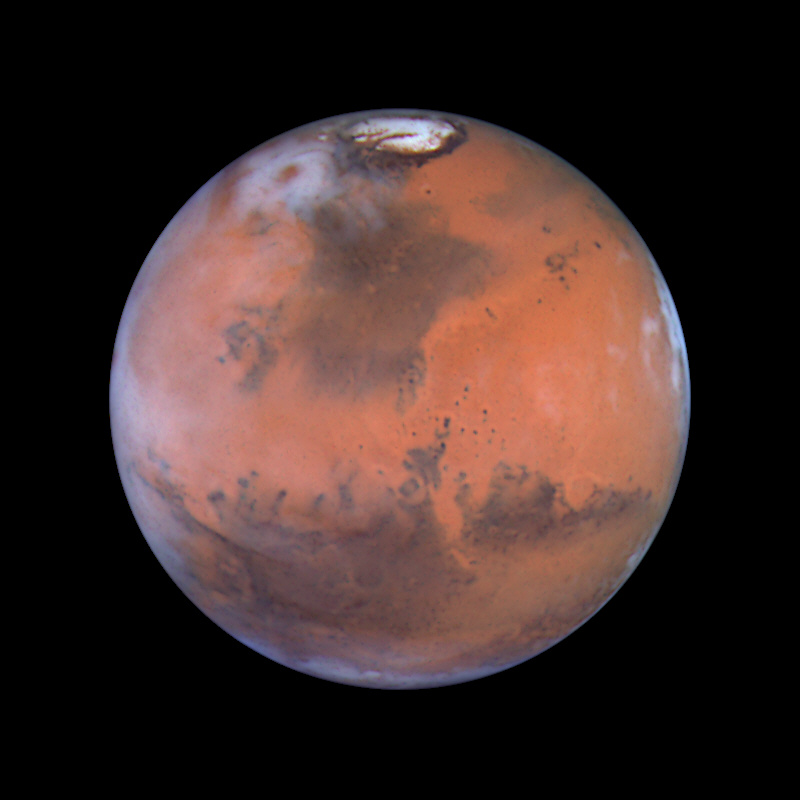
\includegraphics[width=40pt]{mars.jpeg}
        \caption{ Ten rysunek jest w bieżącym miejscu tekstu. Szerokość to 40 punktów tekstu.}
\end{figure}
tortor sit amet semper consectetur, est ipsum commodo lorem, ac suscipit libero massa quis turpis. Interdum et malesuada fames ac ante ipsum primis in faucibus.
\section{Sekcja 2}
Odwołanie do tabeli 1.\ref{tab:tabela}
\section{Sekcja 3}

To przepis na potrawę\footnote{Opracowano na podstawie. \url{https://www.kwestiasmaku.com/zielony_srodek/
salatki_jablka/jablka_pieczone/jablka_pieczone_z_platkami_owsianymi/przepis.
html}} 
Zwróć uwagę na punktory i numerację.

\begin{enumerate}[$\circ$]
\item Składniki - cz.1.
        \begin{enumerate}[I.]
    \item 500 g filetów białej ryby (np. dorsz, morszczuk, mintaj)
    \item 600 g filetów łososia
    \item po 1 łyżeczce kurkumy i papryki słodkiej + szczypta ostrej
    \item 1 łyżka soku z cytryny
    \item 2 łyżki oliwy
        \end{enumerate}
\item Składniki - cz.2.
        \begin{enumerate}[A)]
    \item wanilia 
    \item cukier waniliowy
    \item ziarenka z wanilii
        \end{enumerate}
\item Przygotowanie
        \begin{enumerate}[1.]
\item[1.]Piekarnik nagrzać do 180 stopni C. Ściąć wierzch jabłek, wyciąć/wydrążyć ogryzek, uważając aby nie przeciąć brzegów i skórki jabłek.
\item[2.]Wymieszać płatki owsiane z żurawiną, cynamonem, wanilią i włożyć do środka. Skropić sokiem z limonki lub cytryny.
\item[6.]Na wierzch położyć pokrojone orzechy i polać syropem lub posypać cukrem. Przykryć "pokrywką" z jabłka i wstawić do piekarnika.
\item[7.]Piec przez ok. 30 minut, ale dokładna długość pieczenia zależy od stopnia dojrzałości jabłek, trzeba po prostu sprawdzać.
    \end{enumerate}
\end{enumerate}


\section{Wzory matematyczne}
Tutaj testujemy wzory matematyczne. Wszystkie są wyśrodkowane w oddzielnym wierszu. Zwróć uwagę, że niektóre posiadają numery. Odwołanie
do wzoru 1.\ref{mat:wzo}



\begin{equation*}
\label{eqn:somelabel}
L'=L \sqrt{1-\frac{v^2}{c^2}}
\end{equation*}

\begin{equation*}
u(x)= \left\{ \begin{array}{llcc}
  \exp x & \mbox{if} & x \geq 0
  \\
  1  & \mbox{if} & x < 0
\end{array}\right.
\end{equation*}

\begin{equation}
\left[
\begin{array}{ccc|cc}
     1& 2&3 &7 & 6\\\hline
     2& 4& 6&5 &4
\end{array}
\right]
\end{equation}

\end{document}
